\documentclass[conference]{IEEEtran}
\IEEEoverridecommandlockouts

\usepackage{cite}
\usepackage{amsmath,amssymb,amsfonts}
\usepackage{graphicx}
\graphicspath{{../../results/plots/}{figures/}}
\usepackage{textcomp}
\usepackage{xcolor}
\usepackage{booktabs}
\usepackage[hidelinks]{hyperref}
\usepackage{array}

\def\BibTeX{{\rm B\kern-.05em{\sc i\kern-.025em b}\kern-.08em
    T\kern-.1667em\lower.7ex\hbox{E}\kern-.125emX}}

\begin{document}

\title{Design and Verification of a Direct-Mapped Cache Controller in Verilog\thanks{\protect\href{https://drive.google.com/drive/folders/1WNsOvDRVHSj_vMWKZjpoxVolT6G_y51Q?usp=drive_link}{Technical demonstration video}}}

\author{
    \IEEEauthorblockN{Mustyala Sadhvik}
    \IEEEauthorblockA{2401020099 \\
    \url{musthyala.sadhvik2024@nst.rishihood.edu.in}}
    \and
    \IEEEauthorblockN{Udata Varun}
    \IEEEauthorblockA{2401010481 \\
    \url{udata.varun2024@nst.rishihood.edu.in}}
    \and
    \IEEEauthorblockN{Amogha Raj Sandur}
    \IEEEauthorblockA{2401010397 \\
    \url{s.raj2024@nst.rishihood.edu.in}}
    \and
    \IEEEauthorblockN{Yachna Khanna}
    \IEEEauthorblockA{2401010509 \\
    \url{yachna.2024@nst.rishihood.edu.in}}
    \and
    \IEEEauthorblockN{Shrihari K N}
    \IEEEauthorblockA{2401010448 \\
    \url{shrihari.n2024@nst.rishihood.edu.in}}
}

\maketitle

\begin{abstract}
We implement and evaluate a parameterized, blocking direct-mapped cache for a 32-bit word-oriented CPU interface. The Verilog controller uses write-back, write-allocate, and a four-state finite state machine for lookup, dirty eviction, and refill. Self-checking Icarus Verilog tests cover all 12 cache geometries, including capacities from 1 to 8~KiB and block sizes from 8 to 32~B. Phase~II evaluates sequential, strided, conflict, and random workloads in 48 geometry runs, plus a fixed-geometry latency sweep. At 4~KiB with 16~B blocks and 10-cycle backing memory, sequential achieves 75.00\% hits and an average memory access time (AMAT) of 5.00~cycles/access. Conflict ping-pong incurs 1,022 conflict misses and 256 dirty write-backs at the same geometry. At 8~KiB the two blocks map to different indices and the hit rate reaches 99.80\%. Increasing memory latency from 5 to 50 cycles raises conflict AMAT from 10.50 to 66.75~cycles/access, reflecting the cost of both refills and write-backs.
\end{abstract}

\begin{IEEEkeywords}
Cache memory, direct-mapped cache, write-back, write-allocate, Verilog HDL, memory hierarchy, cache controller FSM.
\end{IEEEkeywords}

\section{Introduction}
\subsection{The Processor-Memory Performance Gap}
Over the past four decades, microprocessor performance scaling has fundamentally outpaced advances in main memory access latency, a phenomenon canonically recognized in computer architecture as the ``memory wall'' \cite{hennessy2019computer, patterson2020computer}. While semiconductor manufacturing techniques and aggressive instruction-level parallelism (superscalar execution, out-of-order execution, deep pipelining) historically drove processor clock frequencies from megahertz to gigahertz regimes, dynamic random-access memory (DRAM) latency has improved by only a modest factor. Consequently, the relative cost of accessing un-cached main memory has expanded from parity to hundreds of processor clock cycles.

In accordance with Amdahl's Law, as arithmetic execution latency diminishes, memory access overhead becomes the dominant constraint on sustained compute throughput. To bridge this performance disparity, computer architects introduce hierarchical memory subsystems, interpolating small, ultra-fast static random-access memory (SRAM) caches between the processor registers and large, higher-latency backing storage. By exploiting spatial and temporal program locality, caches serve the vast majority of CPU memory requests within one or two clock cycles, decoupling processor execution rates from external memory latency.

\subsection{Problem Statement}
Designing an effective Level-1 (L1) cache controller requires careful balancing among access latency, circuit complexity, silicon area, and coherence guarantees. While higher associativity can suppress conflict misses, it introduces parallel tag comparators, wide multiplexing networks, and replacement policy state logic, which can degrade the processor's critical timing path.

The primary objective of this project is to implement a cycle-accurate, fully synthesizable hardware controller in Verilog HDL for a 4~KB direct-mapped cache. The controller must seamlessly interface with a 32-bit processor core and a backing memory exhibiting a fixed 10-cycle transfer latency. The system must accept aligned word operations using byte addresses, 16-byte block transfers, valid and dirty state tracking per cache line, a write-back eviction policy to conserve memory bus bandwidth, write-allocate refills on write misses, and a deterministic four-state finite state machine (FSM) ensuring race-free, blocking protocol handshakes.

\subsection{Design Objectives}
The specific engineering and architectural objectives for this implementation encompass:
\begin{enumerate}
    \item \textbf{Modular RTL Architecture}: Partitioning the microarchitecture into clean, decoupled, and independently verifiable functional modules, including a Tag Array (\texttt{tag\_array.v}), Data Array (\texttt{data\_array.v}), Controller FSM (\texttt{cache\_controller.v}), and Top-Level Cache (\texttt{cache\_top.v}).
    \item \textbf{Strict Specification Conformance}: Adhering rigorously to a 32-bit physical address format segmented into a 20-bit tag, 8-bit index, 2-bit block word offset, and 2-bit byte offset across 256 lines, with a 128-bit block-wide backing memory interface.
    \item \textbf{Rigorous Functional Verification}: Constructing self-checking verification testbenches for each modular block and the integrated subsystem, utilizing open-source EDA tooling (Icarus Verilog and GTKWave) to validate corner cases, boundary conditions, and state transitions.
    \item \textbf{Performance Characterization Framework}: Providing synthetic memory access trace drivers and evaluation scripts to empirically quantify cache hit rates, miss penalties, and Average Memory Access Time (AMAT).
\end{enumerate}

\section{Literature Review}
\subsection{Memory Hierarchy, Locality, and Cache Organizations (M1)}
The effectiveness of cache memory hinges on the empirical phenomenon of program locality, formally characterized in the foundational taxonomy established by Smith \cite{smith1982cache}. Program executions consistently exhibit two distinct operational dimensions of locality:
\begin{itemize}
    \item \textbf{Temporal Locality}: Memory locations accessed in the immediate past possess a high probability of being referenced again in the near future (e.g., loop control variables, active stack frames, inner-loop instructions).
    \item \textbf{Spatial Locality}: Memory locations geographically proximate to recently accessed addresses are highly likely to be referenced shortly thereafter (e.g., sequential instruction streams, array traversals, contiguous data structures).
\end{itemize}

Caches exploit temporal locality by retaining recently referenced data in high-speed SRAM, while exploiting spatial locality by fetching multi-word contiguous blocks (lines) from backing memory upon a miss, rather than individual words or bytes \cite{patterson2020computer}.

Architecturally, cache structures are categorized into three primary placement paradigms based on degree of associativity: direct-mapped, set-associative, and fully associative \cite{hennessy2019computer}.
\begin{enumerate}
    \item \textbf{Direct-Mapped}: Each physical block address maps deterministically to exactly one cache line, governed by the modular relationship:
    \begin{equation}
        \text{Index} = \left\lfloor\frac{\text{Byte Address}}{\text{Block Size}}\right\rfloor \bmod (\text{Number of Lines})
    \end{equation}
    Because only a single tag comparison is required per access, direct-mapped caches require no associative search logic, eliminate replacement decision algorithms (such as LRU or pseudo-LRU), and minimize multiplexer fan-in. In his seminal work, Hill \cite{hill1988case} argued compellingly that direct-mapped caches frequently yield superior overall system performance in timing-critical L1 configurations. When cache hit latency dictates the processor's primary clock cycle period, the critical-path timing advantages of direct-mapped indexing offset the marginally lower miss rates of multi-way associative designs. However, direct-mapped structures remain vulnerable to conflict misses, which occur when multiple actively referenced memory blocks map to the same line index.
    \item \textbf{Set-Associative}: Caches partition storage into sets of $N$ parallel ways ($N \ge 2$). A block maps to a unique set, but may occupy any way within that set. While set-associativity reduces conflict misses, it incurs increased hardware area, dynamic power dissipation, parallel comparator structures, and multiplexing delays on the hit data path \cite{hennessy2019computer}.
    \item \textbf{Fully Associative}: Any memory block may be placed in any cache line. While eliminating conflict misses entirely, fully associative lookup necessitates $S$ simultaneous tag comparisons via content-addressable memory (CAM) structures, rendering it practical only for very small structures such as Translation Lookaside Buffers (TLBs) or victim caches \cite{smith1982cache, jouppi1990improving}.
\end{enumerate}

To mitigate conflict misses inherent to direct-mapped caches without compromising their clock frequency advantages, Jouppi \cite{jouppi1990improving} introduced the victim cache architecture. By positioning a small, fully associative SRAM buffer between the direct-mapped L1 cache and the memory subsystem, evicted clean and dirty blocks are temporarily retained. On a miss in the direct-mapped cache, a secondary parallel lookup in the victim cache allows swift recovery of thrashing blocks, demonstrating that targeted microarchitectural augmentations can retain direct-mapped speed while approaching multi-way hit rates \cite{jouppi1990improving}.

\subsection{Write Policies and Main Memory Interfacing (M2)}
Handling memory write operations efficiently is central to cache microarchitecture because writes introduce consistency obligations between on-chip SRAM and backing main memory \cite{smith1982cache, patterson2020computer}. Two orthogonal design choices govern write behavior: the \emph{write-hit policy} and the \emph{write-miss allocation policy} \cite{hennessy2019computer}.

\begin{itemize}
    \item \textbf{Write-Through vs.\ Write-Back (Write-Hit Policy)}: Under a \emph{write-through} policy, every processor store updates both the cache line and main memory synchronously. Although write-through simplifies hardware state tracking and keeps backing memory continuously up to date, every store consumes external memory bandwidth and risks stalling the CPU unless buffered by a write buffer \cite{patterson2020computer}. Conversely, a \emph{write-back} (copy-back) policy updates only the cache SRAM on a write hit and asserts a per-line \texttt{dirty} bit. Modified lines are transferred back to main memory only when evicted upon a conflicting miss. As characterized by Smith \cite{smith1982cache}, write-back coalesces multiple stores to words within the same block into a single block-wide memory write, dramatically lowering memory bus traffic when backing memory exhibits multi-cycle latency.
    \item \textbf{Write-Allocate vs.\ No-Write-Allocate (Write-Miss Policy)}: Under \emph{write-allocate} (fetch-on-write), a write miss loads the missing block from main memory into the cache before writing the target word. Under \emph{no-write-allocate} (write-around), the store bypasses the cache and updates main memory directly \cite{hennessy2019computer}. Write-allocate pairs naturally with write-back because subsequent reads or writes to neighboring words in the newly fetched block become fast cache hits; conversely, no-write-allocate is typically coupled with write-through \cite{patterson2020computer}.
\end{itemize}

For a blocking cache connected to a backing memory with \texttt{MEM\_LATENCY} $= 10$ cycles over a 128-bit block-wide interface, combining \textbf{write-back} with \textbf{write-allocate} minimizes redundant bus transactions. Each cache line therefore carries a \texttt{dirty} bit alongside its \texttt{valid} bit and tag, requiring the controller to perform a 128-bit \texttt{WRITE\_BACK} prior to \texttt{ALLOCATE} whenever a dirty block is evicted \cite{hennessy2019computer}.

\subsection{Miss classification and improving direct-mapped caches}
A compulsory miss occurs on the first reference to a block. To classify later misses, compare the direct-mapped cache with a fully associative cache of the same capacity and block size, using least-recently-used replacement in the reference cache. A capacity miss also occurs in the reference cache because its limited storage forced the block out. A conflict miss is a miss in the direct-mapped cache that would hit in the reference cache \cite{patterson2020computer}.

A 4~KB direct-mapped cache with 16-byte blocks places addresses \texttt{0x00000028} and \texttt{0x00001028} at the same index. The first access to each block is compulsory. Repeated alternation then causes conflict misses because the two blocks replace each other even though the rest of the cache has room. Increasing associativity allows both blocks to occupy the same set, at the cost of comparing more tags on each lookup \cite{hill1988case}.

Jouppi proposed a small, fully associative victim cache that holds recently evicted lines. When a primary-cache miss hits in the victim cache, the requested block and the line it displaces can swap, avoiding a fetch from backing memory. This approach targets mapping conflicts while preserving the direct-mapped primary lookup \cite{jouppi1990improving}. The Phase~I prototype uses the direct-mapped baseline to expose the cost of those conflicts.

\subsection{Hardware Verification Methodology and Golden Reference Models (M4)}
Functional verification of hardware memory controllers presents unique challenges due to complex multi-cycle handshakes, state-dependent side effects, and asynchronous bus interactions \cite{hennessy2019computer, patterson2020computer}. In modern digital design flows, simulation-based verification remains the principal methodology for validating RTL implementations against microarchitectural specifications prior to physical synthesis \cite{patterson2020computer}.

Effective verification of cache subsystems necessitates a dual-layer strategy combining directed stress testing with reference model checking:
\begin{enumerate}
    \item \textbf{Self-Checking Testbenches}: Traditional manual inspection of waveform traces is inherently error-prone and unscalable. Self-checking testbenches automate validation by encapsulating stimulus generation, response monitoring, and invariant assertion checking directly in Verilog tasks \cite{patterson2020computer}. Bus driver tasks synchronize with clock edges, enforce protocol timing, and incorporate timeout watchdogs to detect protocol deadlocks or stalled handshakes.
    \item \textbf{Golden Reference Models}: To verify functional correctness across sequence-dependent memory operations, the verification environment couples the Device Under Test (DUT) to an independent, high-level reference oracle (the ``golden model'') \cite{hennessy2019computer}. In cache verification, this oracle is implemented as an un-cached, direct-storage software memory array. While the DUT cache handles tagging, indexing, sub-word multiplexing, write-back buffering, and multi-cycle memory latency, the golden reference array updates synchronously on every committed CPU write. On every load transaction, the data returned by the DUT is evaluated concurrently against the golden array. Any divergence immediately exposes data corruption, stale reads, or incorrect replacement logic.
    \item \textbf{Corner-Case and Directed Stimulus}: As classified by Smith \cite{smith1982cache}, cache operations span distinct operational regimes: cold misses, cache hits, sub-word writes, write-allocate refills, clean evictions, and dirty write-backs. Targeted directed sequences systematically exercise boundary lines, index aliasing, and memory latency transitions that random stimulus might fail to trigger.
\end{enumerate}

\subsection{FPGA and Verilog Cache Implementations}
Hill relates direct mapping to the critical path of a cache lookup \cite{hill1988case}. On an FPGA, the achievable hit path also depends on the inferred storage and its read timing. The Verilog tag and data arrays here expose combinational reads. A synchronous block-RAM mapping would require accounting for its registered read in the controller schedule. The block-wide refill, per-word writes, metadata updates, and reset behavior also affect memory inference. A hardware comparison would report the FPGA family, memory resources, achievable frequency, and workload alongside cycle counts. This project measures RTL behavior with a behavioral memory model.

\section{Proposed Solution}
\subsection{System Architecture and Address Decomposition}
The cache subsystem connects a 32-bit processor core (\texttt{req}, \texttt{we}, \texttt{addr}, \texttt{wdata}, \texttt{rdata}, \texttt{ready}) to a 128-bit block-wide backing memory interface (\texttt{mem\_req}, \texttt{mem\_we}, \texttt{mem\_addr}, \texttt{mem\_wdata}, \texttt{mem\_rdata}, \texttt{mem\_ready}). Given \texttt{CACHE\_SIZE} $= 4096$~bytes, \texttt{BLOCK\_SIZE} $= 16$~bytes (four 32-bit words), and direct-mapped placement ($1$ way per set), the cache holds $S = 4096 / 16 = 256$ lines. Accordingly, each 32-bit physical byte address (\texttt{ADDR\_WIDTH} $= 32$) is decomposed into four non-overlapping bit fields:
\begin{itemize}
    \item \textbf{Byte Offset} ($\texttt{addr[1:0]}$, $2$ bits): Addresses an individual byte inside a 4-byte word ($\log_2 4 = 2$).
    \item \textbf{Block Offset} ($\texttt{addr[3:2]}$, $2$ bits): Selects one of the four 32-bit words inside a 16-byte cache line ($\log_2(16/4) = 2$).
    \item \textbf{Index} ($\texttt{addr[11:4]}$, $8$ bits): Directly selects one of the $256$ cache lines in both the Tag Array and Data Array ($\log_2 256 = 8$).
    \item \textbf{Tag} ($\texttt{addr[31:12]}$, $20$ bits): Uniquely identifies which physical memory block currently occupies the indexed line ($32 - (8 + 2 + 2) = 20$).
\end{itemize}

\begin{table}[htbp]
\caption{32-Bit Physical Address Decomposition}
\begin{center}
\begin{tabular}{|l|c|c|p{3.1cm}|}
\hline
\textbf{Field} & \textbf{Bits} & \textbf{Width} & \textbf{Hardware Role} \\
\hline
Tag & \texttt{[31:12]} & 20 & Tag comparator / eviction address \\
\hline
Index & \texttt{[11:4]} & 8 & Selects line $0$--$255$ \\
\hline
Block Offset & \texttt{[3:2]} & 2 & 4:1 word mux / write lane \\
\hline
Byte Offset & \texttt{[1:0]} & 2 & Sub-word alignment \\
\hline
\end{tabular}
\label{tab:addr_split}
\end{center}
\end{table}

For example, address \texttt{0x00012348} splits into Tag \texttt{0x00012}, Index \texttt{0x34} (line~52), Block Offset \texttt{2'b10} (word~2, block bits \texttt{[95:64]}), and Byte Offset \texttt{2'b00}, mapping to the 16-byte aligned memory block starting at \texttt{\{addr[31:4], 4'b0000\} = 0x00012340}.

\begin{figure}[htbp]
\centering
\setlength{\unitlength}{0.72pt}
\scriptsize
\begin{picture}(320,139)
    \put(111,114){\framebox(98,18){CPU interface}}
    \put(103,78){\framebox(114,18){Cache controller}}
    \put(6,43){\framebox(100,18){Tag array}}
    \put(214,43){\framebox(100,18){Data array}}
    \put(103,8){\framebox(114,18){Main memory model}}
    \put(160,109){\vector(0,1){5}}
    \put(160,101){\line(0,1){8}}
    \put(160,101){\vector(0,-1){5}}
    \put(170,105){\makebox(0,0)[l]{Request / response}}
    \put(56,87){\line(1,0){41}}
    \put(97,87){\vector(1,0){6}}
    \put(56,87){\vector(0,-1){26}}
    \put(223,87){\line(1,0){41}}
    \put(223,87){\vector(-1,0){6}}
    \put(264,87){\vector(0,-1){26}}
    \put(52,72){\makebox(0,0)[r]{Metadata}}
    \put(268,72){\makebox(0,0)[l]{Word I/O}}
    \put(160,32){\line(0,1){40}}
    \put(160,72){\vector(0,1){6}}
    \put(160,32){\vector(0,-1){6}}
    \put(167,48){\makebox(0,0)[l]{Control}}
    \put(264,17){\line(0,1){20}}
    \put(264,37){\vector(0,1){6}}
    \put(264,17){\vector(-1,0){47}}
    \put(261,5){\makebox(0,0){128-bit block I/O}}
\end{picture}
\caption{Block diagram of the integrated cache subsystem.}
\label{fig:cache_m3_architecture}
\end{figure}

Figure~\ref{fig:cache_m3_architecture} shows the four modules instantiated by \texttt{cache\_top}. The controller latches one CPU request, supplies its index to both arrays, and uses the stored metadata to determine whether the selected line can serve that request. The data array exchanges a 32-bit word with the controller and a full 128-bit block with the memory model. A store updates one word, while a refill writes all four words. The memory model reports each completed block transfer to the controller through \texttt{mem\_ready}.

\subsection{Tag Array Subsystem Design}
The Tag Array (\texttt{rtl/tag\_array.v}) stores per-line metadata across $256$ entries: a 20-bit tag (\texttt{tag\_mem}), a 1-bit validity flag (\texttt{valid\_mem}), and a 1-bit modification flag (\texttt{dirty\_mem}). Asynchronous continuous reads expose \texttt{tag\_out}, \texttt{valid\_out}, and \texttt{dirty\_out} in the same cycle as \texttt{index} presentation, enabling single-cycle hit evaluation (\texttt{hit = valid\_out \&\& (tag\_out == addr[31:12])}) during \texttt{COMPARE\_TAG}. Synchronous active-high \texttt{rst} clears all 256 valid, dirty, and tag entries. On miss allocation, \texttt{write\_en} loads \texttt{tag\_in}, \texttt{valid\_in}, and \texttt{dirty\_in} on the rising clock edge; on CPU write hits, \texttt{set\_dirty} marks the indexed line dirty without overwriting its tag or valid state.

\subsection{Data Storage Array and Sub-word Multiplexing}
The Data Array (\texttt{rtl/data\_array.v}) implements the 4~KB cache payload as a $256 \times 128$-bit synchronous memory array (\texttt{data\_mem}), holding four 32-bit words per line in little-endian word order: Word~0 in \texttt{[31:0]}, Word~1 in \texttt{[63:32]}, Word~2 in \texttt{[95:64]}, and Word~3 in \texttt{[127:96]}. On the read datapath, combinational indexing drives \texttt{block\_out[127:0]} directly for 128-bit dirty evictions while a 4:1 multiplexer controlled by \texttt{word\_offset} (\texttt{addr[3:2]}) routes the target 32-bit word to \texttt{word\_out[31:0]}. On the write datapath, asserting \texttt{write\_block\_en} refills an entire 128-bit line from \texttt{block\_in} during \texttt{ALLOCATE} (taking precedence if both write enables are high), whereas asserting \texttt{write\_word\_en} updates only the 32-bit word selected by \texttt{word\_offset} with \texttt{word\_in} while preserving the remaining three words in the block. Synchronous \texttt{rst} clears all 256 lines to zero.

\subsection{Finite State Machine Control Logic}
Figure~\ref{fig:cache_m3_fsm} and Table~\ref{tab:cache_m3_fsm} show how the controller serves one outstanding CPU request. In \texttt{IDLE}, it latches \texttt{addr}, \texttt{we}, and \texttt{wdata}. The latched address selects the same index throughout the request. In \texttt{COMPARE\_TAG}, a hit requires a valid line and an equal tag. On a read hit the array supplies the selected word. On a write hit the array writes the selected word and sets the dirty bit at the clock edge that samples \texttt{ready}.

\begin{figure}[htbp]
\centering
\setlength{\unitlength}{0.72pt}
\scriptsize
\begin{picture}(320,156)
    \put(110,132){\framebox(100,20){\texttt{IDLE}}}
    \put(110,82){\framebox(100,20){\texttt{COMPARE\_TAG}}}
    \put(8,22){\framebox(100,20){\texttt{ALLOCATE}}}
    \put(212,22){\framebox(100,20){\texttt{WRITE\_BACK}}}
    \put(143,132){\vector(0,-1){30}}
    \put(178,102){\vector(0,1){30}}
    \put(135,117){\makebox(0,0)[r]{Latch request}}
    \put(186,117){\makebox(0,0)[l]{Complete on hit}}
    \put(122,82){\vector(-2,-1){80}}
    \put(86,42){\vector(2,1){80}}
    \put(192,82){\vector(2,-1){80}}
    \put(212,32){\vector(-1,0){104}}
    \put(88,70){\makebox(0,0)[r]{Clean / invalid miss}}
    \put(127,50){\makebox(0,0)[l]{Refill done}}
    \put(235,67){\makebox(0,0)[l]{Dirty miss}}
    \put(160,21){\makebox(0,0){Write-back done}}
\end{picture}
\caption{Cache controller transitions. Reset enters \texttt{IDLE}. The transition table includes the wait conditions.}
\label{fig:cache_m3_fsm}
\end{figure}

\begin{table}[htbp]
\caption{Cache controller transitions and actions}
\label{tab:cache_m3_fsm}
\centering
\scriptsize
\setlength{\tabcolsep}{2pt}
\begin{tabular}{@{}p{0.26\columnwidth}
    >{\raggedright\arraybackslash}p{0.18\columnwidth}
    p{0.26\columnwidth}
    >{\raggedright\arraybackslash}p{0.23\columnwidth}@{}}
\toprule
State & Condition & Next state & Actions / outputs \\
\midrule
Any & Reset & \texttt{IDLE} & Clear controller and cache metadata. \\
\texttt{IDLE} & No request & \texttt{IDLE} & Wait. \\
\texttt{IDLE} & Request & \texttt{COMPARE\_TAG} & Latch CPU operands. \\
\texttt{COMPARE\_TAG} & Read hit & \texttt{IDLE} & Return word and assert ready. \\
\texttt{COMPARE\_TAG} & Write hit & \texttt{IDLE} & Write word, mark dirty, assert ready. \\
\texttt{COMPARE\_TAG} & Miss, dirty victim & \texttt{WRITE\_BACK} & Signal miss and dirty eviction. \\
\texttt{COMPARE\_TAG} & Miss, clean or invalid victim & \texttt{ALLOCATE} & Signal miss. \\
\texttt{WRITE\_BACK} & Memory busy & \texttt{WRITE\_BACK} & Hold victim write request. \\
\texttt{WRITE\_BACK} & Memory ready & \texttt{ALLOCATE} & Advance to refill. \\
\texttt{ALLOCATE} & Memory busy & \texttt{ALLOCATE} & Hold requested block read. \\
\texttt{ALLOCATE} & Memory ready & \texttt{COMPARE\_TAG} & Fill data, install valid clean tag, retry. \\
\bottomrule
\end{tabular}
\end{table}

A miss with a valid, dirty victim first writes the full block to the address formed from the stored tag, index, and zeroed block-offset bits. The refill uses the requested tag with the same index and zero offset. When \texttt{mem\_ready} is high in \texttt{ALLOCATE}, both arrays capture the refill on the same edge. The replay then completes through the normal hit path. On a write miss this sequence preserves the remaining words from memory and marks the updated line dirty.

The controller is Mealy because \texttt{ready} depends on the tag comparison in \texttt{COMPARE\_TAG}, and the array fill enables depend on \texttt{mem\_ready} in \texttt{ALLOCATE}. The memory request and transfer direction depend on state. The debug signals report the initial lookup once per request, so a refill replay completes without adding a hit to the trace statistics.

\subsection{Main Memory Interfacing and Latency Handshake}
The backing memory model (\texttt{rtl/main\_memory.v}) simulates a 256~KB word-addressed main memory (\texttt{MEM\_SIZE\_WORDS} $= 65536$) preloaded at simulation startup via \texttt{\$readmemh} from \texttt{traces/mem\_init.hex} (with each word initialized deterministically to its word address). All cache-to-memory transactions transfer an aligned block of \texttt{BLOCK\_SIZE} bytes (\texttt{DATA\_WIDTH} $= \texttt{BLOCK\_SIZE} \times 8$ bits; 16~bytes / 128~bits by default), ignoring the low \texttt{OFFSET\_BITS} address bits so any unaligned address resolves to its enclosing aligned block. Internally, a three-state handshake controller (\texttt{S\_IDLE}, \texttt{S\_WAIT}, \texttt{S\_DONE}) latches \texttt{mem\_addr}, \texttt{mem\_we}, and \texttt{mem\_wdata} when \texttt{mem\_req} asserts, counts \texttt{MEM\_LATENCY} $= 10$ clock cycles, executes the block write or read across all $\texttt{BLOCK\_SIZE}/4$ words, and pulses \texttt{mem\_ready} for exactly one clock cycle. Because \texttt{S\_DONE} ignores trailing \texttt{mem\_req} assertions on the completion cycle, a Moore cache controller can transition directly from \texttt{WRITE\_BACK} to \texttt{ALLOCATE} without spurious re-triggering, and synchronous \texttt{rst} resets only the controller FSM while preserving preloaded memory contents.

\subsection{Parameterized Design}
To evaluate architectural trade-offs across cache capacities ($\texttt{CACHE\_SIZE} \in \{1024, 2048, 4096, 8192\}$~bytes) and line sizes ($\texttt{BLOCK\_SIZE} \in \{8, 16, 32\}$~bytes), all five RTL modules (\texttt{tag\_array}, \texttt{data\_array}, \texttt{cache\_controller}, \texttt{cache\_top}, and \texttt{main\_memory}) compute their storage geometry via \texttt{\$clog2} and \texttt{localparam} derivations \cite{hennessy2019computer, patterson2020computer}:
Let $C_s$ and $B_s$ be the cache capacity and block size in bytes. The line count $n$, offset width $o$, index width $i$, tag width $t$, and transfer width $d$ in bits are
\begin{align}
n &= C_s/B_s, & o &= \log_2 B_s, & i &= \log_2 n,\\
t &= 32-i-o, & d &= 8 B_s.
\end{align}
Because a direct-mapped cache has one way per set, $\texttt{INDEX\_BITS} + \texttt{OFFSET\_BITS} = \log_2(\texttt{CACHE\_SIZE})$ holds identically across block sizes. Consequently, \texttt{TAG\_BITS} depends solely on total capacity ($22$, $21$, $20$, and $19$~bits for $1$, $2$, $4$, and $8$~KB), while doubling \texttt{BLOCK\_SIZE} at fixed capacity transfers one bit from \texttt{INDEX\_BITS} to \texttt{OFFSET\_BITS}, halves \texttt{NUM\_LINES}, and doubles the memory transfer bus \texttt{DATA\_WIDTH} ($64$, $128$, and $256$~bits). Conversely, doubling \texttt{CACHE\_SIZE} at fixed block size doubles \texttt{NUM\_LINES} and shifts one bit from \texttt{TAG\_BITS} into \texttt{INDEX\_BITS}. Both \texttt{data\_array} (word multiplexing and masked single-word write via indexed part-select) and \texttt{main\_memory} (word-loop packing across $\texttt{BLOCK\_SIZE}/4$ words) scale automatically with \texttt{-P} overrides while preserving identical default behavior at $(4096, 16)$.

\begin{table}[htbp]
\caption{Derived Address Bit Widths and Line Counts Across All 12 Configurations}
\label{tab:param_configs}
\centering
\scriptsize
\setlength{\tabcolsep}{3.5pt}
\begin{tabular}{|c|c|c|c|c|c|c|}
\hline
\textbf{Cache} & \textbf{Block} & \textbf{Lines} & \textbf{Tag} & \textbf{Index} & \textbf{Offset} & \textbf{Data Bus} \\
\textbf{(B)} & \textbf{(B)} & (\texttt{NUM\_LINES}) & \textbf{(b)} & \textbf{(b)} & \textbf{(b)} & \textbf{(b)} \\
\hline
1024 & 8  & 128  & 22 & 7  & 3 & 64  \\
1024 & 16 & 64   & 22 & 6  & 4 & 128 \\
1024 & 32 & 32   & 22 & 5  & 5 & 256 \\
\hline
2048 & 8  & 256  & 21 & 8  & 3 & 64  \\
2048 & 16 & 128  & 21 & 7  & 4 & 128 \\
2048 & 32 & 64   & 21 & 6  & 5 & 256 \\
\hline
4096 & 8  & 512  & 20 & 9  & 3 & 64  \\
\textbf{4096} & \textbf{16} & \textbf{256} & \textbf{20} & \textbf{8} & \textbf{4} & \textbf{128} \\
4096 & 32 & 128  & 20 & 7  & 5 & 256 \\
\hline
8192 & 8  & 1024 & 19 & 10 & 3 & 64  \\
8192 & 16 & 512  & 19 & 9  & 4 & 128 \\
8192 & 32 & 256  & 19 & 8  & 5 & 256 \\
\hline
\end{tabular}
\end{table}

\subsection{Verification Architecture and Test Plan Design (M4)}
To guarantee functional compliance, we construct an automated, self-checking verification environment in \texttt{tb/tb\_cache.v} and \texttt{tb/tb\_directed.v}, structured according to the test plan in \texttt{docs/test\_plan.md}. The verification infrastructure is organized around three design pillars:
\begin{enumerate}
    \item \textbf{Synchronous Bus Driver Tasks}: Reusable Verilog tasks (\texttt{cpu\_read} and \texttt{cpu\_write}) emulate processor load and store transactions. The tasks drive \texttt{req}, \texttt{we}, \texttt{addr}, and \texttt{wdata} on negative clock edges and sample the cache's Mealy \texttt{ready} strobe on positive edges, ensuring race-free handshakes.
    \item \textbf{Protocol Timeout Watchdogs}: Each bus transaction task includes a loop counter that trips if the cache controller fails to assert \texttt{ready} within $250$ clock cycles, preventing simulation deadlocks and pinpointing stalled states.
    \item \textbf{Golden Reference Model}: A $65536 \times 32$-bit software array (\texttt{golden\_mem}) preloaded with \texttt{traces/mem\_init.hex} provides an independent reference oracle. Every write transaction updates \texttt{golden\_mem[addr[17:2]]}, and every read transaction compares \texttt{rdata} against the oracle to immediately detect stale reads, eviction corruptions, or aliasing bugs.
\end{enumerate}

\section{Results and Discussion}

\subsection{Functional Verification and Waveforms}
Icarus Verilog ran the self-checking unit, integration, and parameter testbenches. The tag-array, data-array, and backing-memory unit tests passed 271, 283, and 42 checks, respectively. The golden-memory test passed all nine transactions, the directed suite passed 60 assertions across eight cases, and the corner-case suite passed all eight cases. The latter exercises reset during allocation, a sustained request across completion, dirty conflicts, and consecutive hits. The parameter test passed all 12 geometries, including read-back after a dirty eviction. The repository records these results in \texttt{results/m4\_regression.log} and \texttt{results/param\_check.log}.

Figure~\ref{fig:directed-waves} plots simulation signals from \texttt{tb\_directed}. For the cold read at \texttt{0x00000028}, the initial miss pulses at 65~ns. The controller requests block \texttt{0x00000020} at 75~ns, memory raises \texttt{mem\_ready} at 175~ns, and replay raises CPU \texttt{ready} at 185~ns with data \texttt{0x0000000a}. The repeated read pulses \texttt{hit} and \texttt{ready} together at 215~ns, with \texttt{mem\_req} low. In TC-07, the dirty eviction raises \texttt{dirty\_evict} at 1145~ns. At 1155~ns, the controller requests a write to victim block \texttt{0x00000020}. At 1265~ns, the direction switches to a refill of block \texttt{0x00001020}. CPU \texttt{ready} rises at 1375~ns. Later reads of the original block verify the evicted values, including \texttt{0xDEADBEEF} at \texttt{0x00000028}.

\begin{figure*}[!t]
\centering
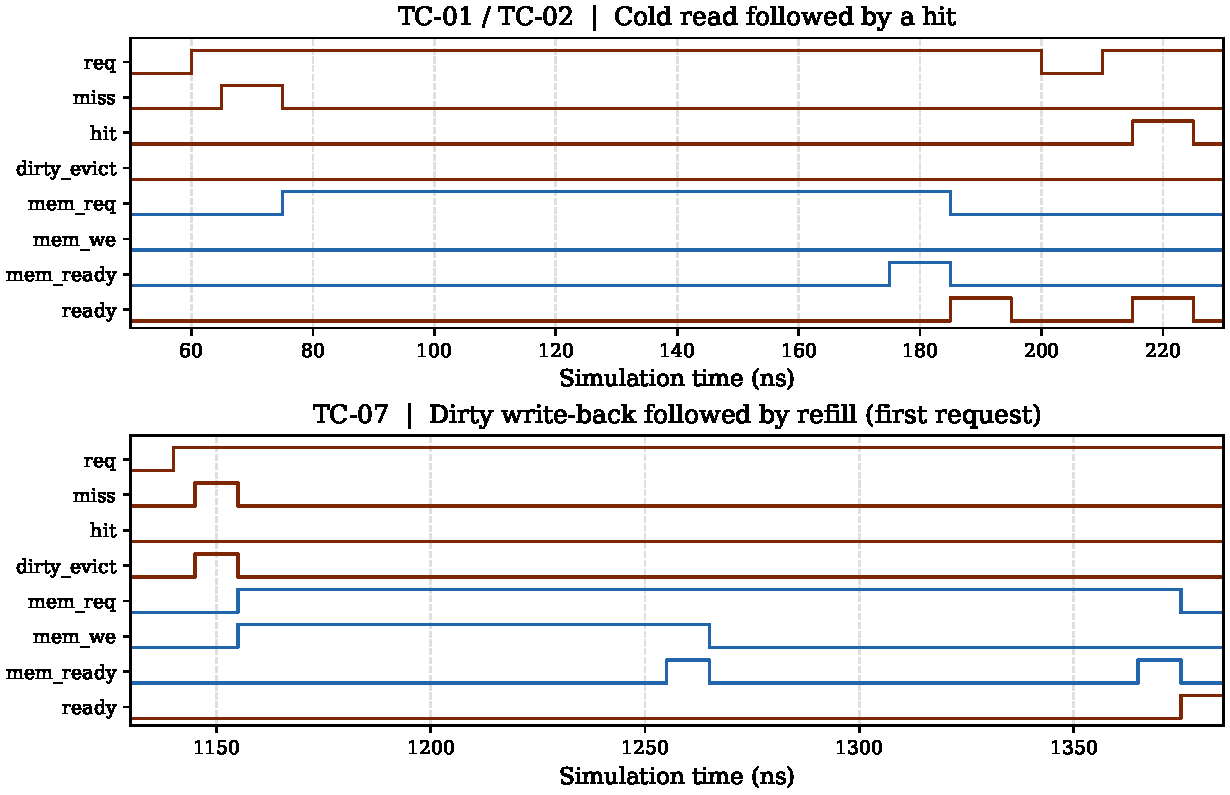
\includegraphics[width=.74\textwidth]{directed_waveforms.pdf}
\caption{Signals captured from the directed RTL testbench. Top: a cold refill followed by a hit. Bottom: the first request in the dirty eviction test. The clock period is 10~ns.}
\label{fig:directed-waves}
\end{figure*}

\subsection{Workloads and Measurement}
Each run starts with a cold cache and issues 1,024 operations. Sequential reads consecutive words. Strided reads 512 addresses 16~B apart, then alternates 512 times between \texttt{0x2000} and \texttt{0x3000}. Conflict ping-pong alternates between \texttt{0x0000} and \texttt{0x1000} with a write every fourth request starting with the first. Random samples aligned addresses over 16~KiB using seed~42 and selects writes with probability $1/4$.

We ran all 48 workload--geometry pairs at $L=10$ cycles using capacities of 1, 2, 4, and 8~KiB and block sizes of 8, 16, and 32~B. A second sweep used $L=5,10,20,50$ at 4~KiB and 16~B. The shared 10-cycle points come from the geometry sweep. The RTL counts the initial lookup once and counts a write-back when the memory write handshake completes. The trace testbench checks architectural read data and the hardware counters against an independent model. The software 3Cs classifier checks first references, then probes an equal-line-count fully associative LRU cache on each direct-mapped miss. It updates the reference cache on every access and reproduces the RTL access, hit, and miss counts for all 48 geometry rows.

For $N$ accesses, $M$ misses, and $C$ measured cycles, the hit path takes two counted edges, for capture and completion. One additional edge precedes the first request. For $M>0$, the mean additional miss penalty and AMAT are
\begin{align}
P_{\mathrm{miss}} &= (C-1-2N)/M,\\
\mathrm{AMAT} &= 2+(M/N)P_{\mathrm{miss}}=(C-1)/N .
\end{align}
The miss penalty includes refill, controller overhead, and dirty write-back. With zero misses, AMAT equals the two-cycle hit time. For sequential at 4~KiB and 16~B, $C=5121$ and $M=256$, so $P_{\mathrm{miss}}=12$ cycles and AMAT is 5.00~cycles/access.

\subsection{Geometry Sweep and Miss Classes}
Table~\ref{tab:baseline} gives measured counters, classified misses, and computed AMAT at the baseline. Figure~\ref{fig:hit-slices} shows the two geometry cuts, and Fig.~\ref{fig:amat-grid} shows all 48 AMAT values. The raw counters and AMAT calculations are archived in \texttt{results/sweep\_all\_traces.csv} and \texttt{results/param\_sweeps\_amat.csv}. Miss classes are in \texttt{results/miss\_classification.csv}.

\begin{table*}[!t]
\caption{Baseline Results at 4~KiB, 16~B Blocks, and 10-Cycle Memory Latency. Each Workload Issues 1,024 Requests.}
\label{tab:baseline}
\centering
\small
\setlength{\tabcolsep}{5pt}
\begin{tabular}{@{}lrrrrrrrrr@{}}
\toprule
Workload & Hits & Misses & Hit rate & Write-backs & Compulsory & Conflict & Capacity & Cycles & AMAT (cycles/access) \\
\midrule
Sequential & 768 & 256 & 75.00\% & 0 & 256 & 0 & 0 & 5,121 & 5.00 \\
Strided & 0 & 1,024 & 0.00\% & 0 & 514 & 510 & 0 & 14,337 & 14.00 \\
Conflict ping-pong & 0 & 1,024 & 0.00\% & 256 & 2 & 1,022 & 0 & 17,153 & 16.75 \\
Random & 195 & 829 & 19.04\% & 171 & 644 & 52 & 133 & 13,878 & 13.55 \\
\bottomrule
\end{tabular}
\end{table*}

\begin{figure*}[!tb]
\centering
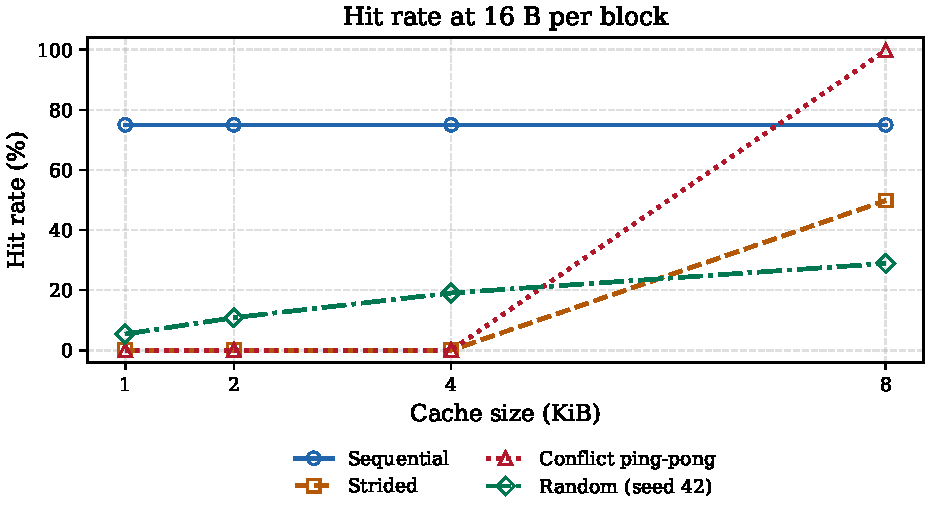
\includegraphics[width=.485\textwidth]{hit_rate_vs_cache_size.pdf}\hfill
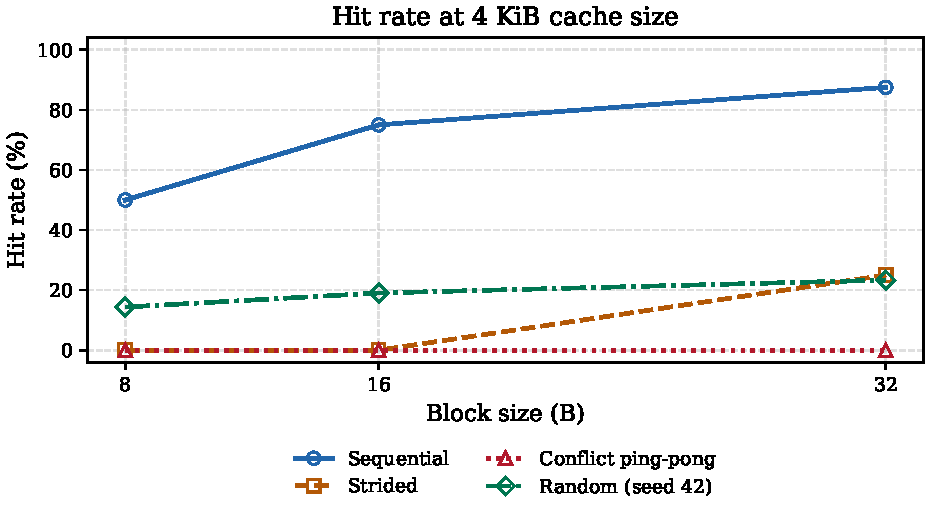
\includegraphics[width=.485\textwidth]{hit_rate_vs_block_size.pdf}
\par\smallskip
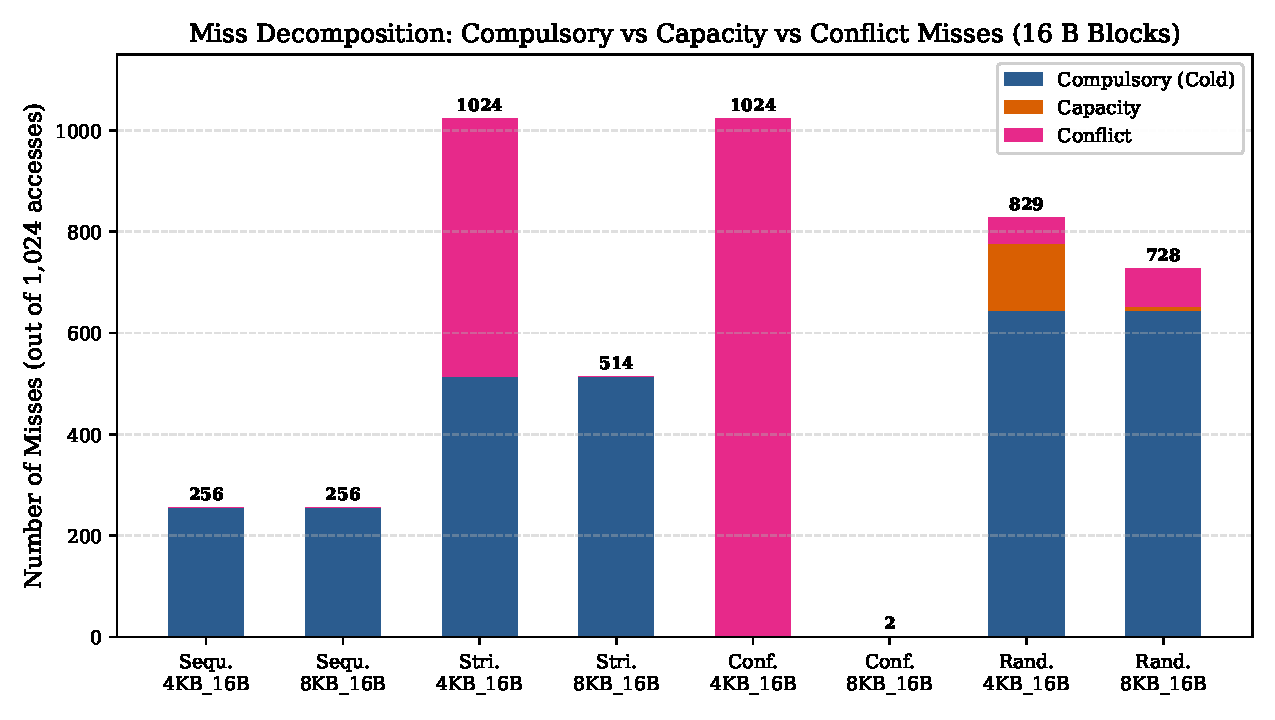
\includegraphics[width=.46\textwidth]{miss_classification_breakdown.pdf}\hfill
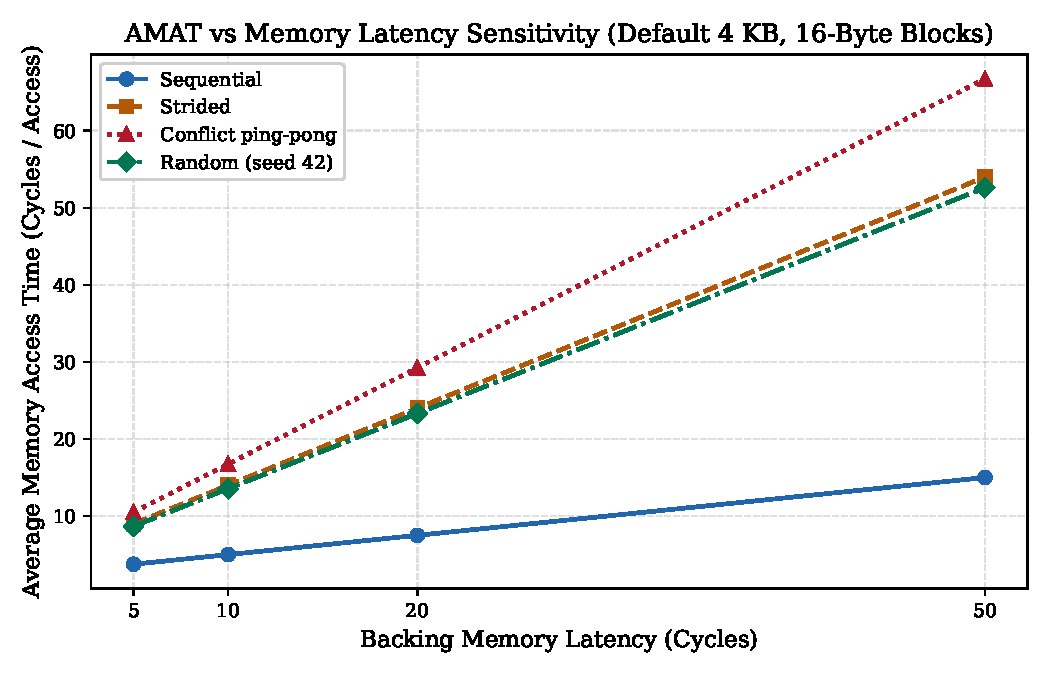
\includegraphics[width=.43\textwidth]{amat_vs_latency.pdf}
\caption{Top: hit rates at 10-cycle memory latency, scanning cache size at 16~B per block (left) and block size at 4~KiB (right). Bottom: 3Cs miss counts at 16~B (left) and AMAT versus backing-memory latency at 4~KiB and 16~B (right).}
\label{fig:hit-slices}
\end{figure*}

\begin{figure}[!t]
\centering
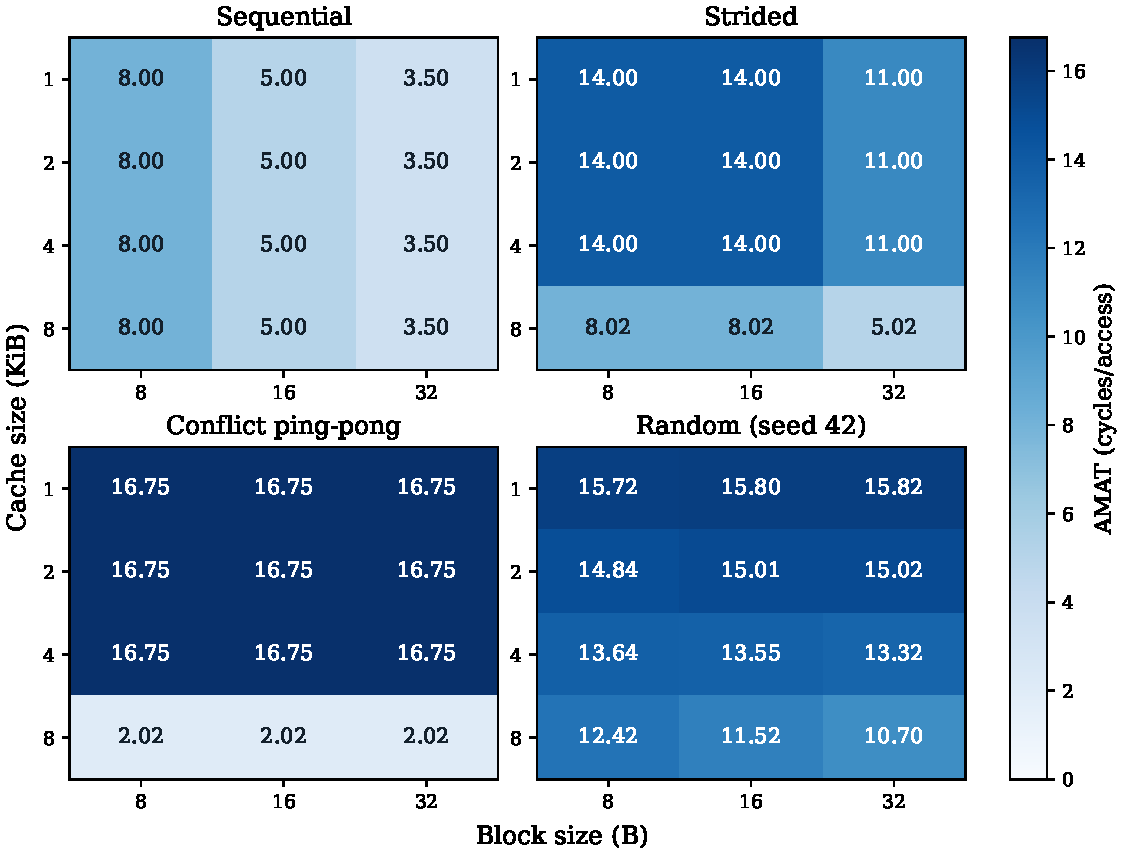
\includegraphics[width=\columnwidth]{amat_by_config.pdf}
\caption{Measured AMAT in cycles/access over the geometry grid at 10-cycle memory latency.}
\label{fig:amat-grid}
\end{figure}

Sequential's 16~B line contains four words. One compulsory miss brings in the next three words, yielding 768 hits and 256 misses. As blocks widen from 8 to 16 to 32~B, the hit rate rises from 50.00\% to 75.00\% to 87.50\%. The gain per doubling shrinks from 25 to 12.5 percentage points. Capacity has no effect on the measured sequential hit rate for any block size because the stream consumes each line before advancing to new addresses.

At 4~KiB, the strided workload stays at 0.00\% through 16~B. At 32~B, two successive 16~B-spaced references in the first half share a block, yielding 256 hits and a 25.00\% hit rate. The 510 conflict misses in its second half remain. For random at 4~KiB, hit rate increases from 14.36\% to 23.34\% from 8 to 32~B. Compulsory misses fall from 800 to 442, but the number of lines falls from 512 to 128 and classified capacity misses rise from 23 to 273. At 1~KiB, random gains just six hits from 8 to 32~B while dirty write-backs rise from 218 to 234. Its AMAT increases from 15.72 to 15.82~cycles/access despite the higher hit rate.

The conflict trace has 0.00\% hits and 1,022 conflict misses from 1 through 4~KiB at 16~B. The address separation is 4,096~B, so both block numbers map to index zero at those sizes. At 8~KiB, the same addresses map to indices 0 and 256. Only two compulsory misses remain, hit rate reaches 99.80\%, and AMAT falls from 16.75 to 2.02~cycles/access. Figure~\ref{fig:hit-slices} shows the miss counts. The two blocks occupy just 32~B at the baseline, which suggests that a two-way set or a one-entry victim cache could retain both blocks after warm-up \cite{jouppi1990improving}. This inference concerns the measured alternating pattern. Both architectures remain future work.

\subsection{Sensitivity to Memory Latency}
At a fixed geometry, the 5-, 10-, 20-, and 50-cycle runs give identical hit, miss, and write-back counts per workload. Each extra memory cycle increases AMAT by $(M+W)/N$, where $W$ is the number of completed dirty write-backs. From 5 to 50~cycles, sequential increases from 3.75 to 15.00~cycles/access with a slope of 0.25, and strided increases from 9.00 to 54.00 with a slope of 1.00. Conflict increases from 10.50 to 66.75 with a slope of 1.25 because it incurs 1,024 refills and 256 write-backs. Random increases from 8.67 to 52.61 with a slope of $1000/1024$ because its 829 refills and 171 write-backs nearly equal the strided transfer count. These values come from \texttt{results/latency\_sweep.csv} and \texttt{results/amat\_table.csv}.



\section{Individual Contributions}
Table~\ref{tab:contributions} selects representative entries from \texttt{git log --format='\%an | \%s'} on the final history. Display names follow the report author list.

\begin{table}[!t]
\caption{Representative Commit Subjects}
\label{tab:contributions}
\centering
\small
\begin{tabular}{@{}cp{.82\columnwidth}@{}}
\toprule
Member & Git history evidence \\
\midrule
M1 & \texttt{07ee4a7} test: corner-case testbench \\
M2 & \texttt{dfe1f5d} feat(mem): block-wide memory by BLOCK\_SIZE \\
M3 & \texttt{ffab70c} feat(amat): calculate access time from measured trace cycles \\
M4 & \texttt{6afe24b} results: miss classification analysis and breakdown for direct-mapped configurations \\
M5 & \texttt{6eb7604} results: cache-size and block-size sweeps \\
\bottomrule
\end{tabular}
\end{table}

\textbf{M1, Mustyala Sadhvik.} Established the repository and IEEEtran source, documented the address split, and implemented the tag array and its unit test. In Phase~II, added eight corner-case scenarios and documented reset and request handshakes.

\textbf{M2, Udata Varun.} Built the data array and backing-memory model with unit tests. Parameterized the arrays and transfers, then added the geometry test and single-trace sweep runner.

\textbf{M3, Amogha Raj Sandur.} Implemented the controller FSM, integrated the top level, and added the smoke test. Added deterministic workloads, measured the latency sweep, and computed AMAT from elapsed RTL cycles.

\textbf{M4, Yachna Khanna.} Built the golden-memory and directed testbenches, simulation runner, and waveform guide. Ran the Phase~II regressions and geometry grid, implemented the 3Cs classifier, and plotted the first evaluation figures.

\textbf{M5, Shrihari K N.} Implemented the performance counters and the initial self-checking sequential trace replay. Repeated the final grid and latency experiments, produced the final figures and waveform excerpts, and completed the report and viva guide.


\section{Conclusion and Future Work}
The parameterized Verilog cache passed the directed, corner-case, and geometry tests. At 4~KiB and 16~B, sequential reaches 75.00\% hits and 5.00~cycles/access, while conflict ping-pong produces 1,022 conflict misses and 16.75~cycles/access. Mapping the alternating addresses to separate lines at 8~KiB reduces that workload's AMAT to 2.02~cycles/access. The latency sweep shows that the number of backing-memory transfers, including dirty write-backs, determines the AMAT slope in this blocking design.

The cache blocks while a miss is in flight, accepts only one outstanding request, and has one way per set. Its fixed mapping gives it no choice of victim and therefore no replacement policy. The evaluation uses synthetic traces and a fixed-latency behavioral memory. Future work can add set associativity with LRU replacement, evaluate a small victim cache for repeated conflicts, and test stream prefetching for predictable accesses. FPGA synthesis would quantify resource use and hit-path timing alongside these cycle counts.

\bibliographystyle{IEEEtran}
\bibliography{references}

\end{document}
